\documentclass[hydrology,article,submit,pdftex,moreauthors]{../MDPI_template_ACS/Definitions/mdpi}

%------------------------------------------------------------------
% MDPI metadata
\firstpage{1}
\makeatletter
\setcounter{page}{\@firstpage}
\makeatother
\pubvolume{1}
\issuenum{1}
\articlenumber{0}
\pubyear{2025}
\copyrightyear{2025}
\datereceived{}
\daterevised{}
\dateaccepted{}
\datepublished{}
\hreflink{https://doi.org/}

%------------------------------------------------------------------
% Additional packages
\usepackage{siunitx}
\usepackage{tikz}
\usetikzlibrary{arrows.meta,positioning,calc,shapes.multipart}
\usepackage{subcaption}
\captionsetup[subfigure]{font=footnotesize,justification=centering,singlelinecheck=false}

% Figures: Overleaf-like layout plus native notebook outputs
\graphicspath{%
  {figures/}{figures/h6/}{figures/h12/}%
  {../../h6/}{../../h12/}%
  {../../../../../models/output/V2_Enhanced_Models/comparisons/}%
  {../../../../../models/output/}%
  {../../../../analysis/}%
}

%------------------------------------------------------------------
% Title, authors, affiliations
\Title{Hybrid Data-Driven Framework for Multi-Month Precipitation Forecasting over Boyac\'a with CHIRPS and DEM Context in Light Mode}
\TitleCitation{Hybrid Data-Driven Framework for Precipitation Forecasting}

\newcommand{\orcidauthorA}{0009-0003-2963-1631}
\newcommand{\orcidauthorB}{0000-0003-1656-4452}
\newcommand{\orcidauthorC}{0000-0002-7396-8915}

\Author{Manuel Ricardo P\'erez Reyes $^{1,2}$\orcidA{}, Marco Javier Su\'arez Bar\'on $^{2}$\orcidB{} and \'Oscar Javier Garc\'ia Cabrejo $^{3}$\orcidC{}}
\AuthorNames{Manuel Ricardo P\'erez Reyes, Marco Javier Su\'arez Bar\'on and \'Oscar Javier Garc\'ia Cabrejo}
\AuthorCitation{P\'erez Reyes, M.R.; Su\'arez Bar\'on, M.J.; Garc\'ia Cabrejo, \'O.J.}
\address{%
$^{1}$ \quad Doctoral Program in Engineering, Pedagogical and Technological University of Colombia (UPTC), Sogamoso 152210, Colombia\\
$^{2}$ \quad Pedagogical and Technological University of Colombia (UPTC), School of Systems Engineering, Sogamoso 152210, Colombia\\
$^{3}$ \quad Pedagogical and Technological University of Colombia (UPTC), School of Geology, Sogamoso 152210, Colombia}
\corres{Correspondence: manuelricardo.perez@uptc.edu.co}

%------------------------------------------------------------------
% Header and footer customization (Hydrology style)
\setlength{\headheight}{20pt}
\fancyhead[L]{}
\fancyhead[C]{}
\fancyhead[R]{\thepage/\pageref{LastPage}\hspace{0.5em}\includegraphics[height=12pt]{Definitions/logo-mdpi-eps-converted-to.pdf}}
\fancyfoot[L]{\footnotesize\textit{Hydrology} 2025, 12, 19}
\fancyfoot[C]{}
\fancyfoot[R]{\footnotesize\href{https://doi.org/10.3390/hydrology1010000}{https://doi.org/10.3390/hydrology1010000}}
\fancypagestyle{plain}{%
  \fancyhf{}
  \fancyhead[L]{}
  \fancyhead[C]{}
  \fancyhead[R]{\thepage/\pageref{LastPage}\hspace{0.5em}\includegraphics[height=12pt]{Definitions/logo-mdpi-eps-converted-to.pdf}}
  \fancyfoot[L]{\footnotesize\textit{Hydrology} 2025, 12, 19}
  \fancyfoot[C]{}
  \fancyfoot[R]{\footnotesize\href{https://doi.org/10.3390/hydrology1010000}{https://doi.org/10.3390/hydrology1010000}}
  \renewcommand{\headrulewidth}{0.4pt}
  \renewcommand{\footrulewidth}{0pt}
}
\fancypagestyle{titlepage}{%
  \fancyhf{}
  \fancyhead[L]{\includegraphics[height=36pt]{figures/hydrology-logo-print.png}}
  \fancyhead[C]{}
  \fancyhead[R]{\includegraphics[height=12pt]{Definitions/logo-mdpi-eps-converted-to.pdf}}
  \renewcommand{\headrulewidth}{0.4pt}
  \renewcommand{\footrulewidth}{0pt}
}
\pagestyle{fancy}
\renewcommand{\headrulewidth}{0.4pt}
\renewcommand{\footrulewidth}{0pt}

%------------------------------------------------------------------
% Abstract and keywords
\abstract{%
Background: Reliable multi-month precipitation forecasts underpin flood and drought preparedness in mountainous regions. We present a hybrid data-driven framework that couples CHIRPS v2.0 precipitation with a Boyac\'a DEM, orchestrating feature bundles and lightweight architectures in a light-mode setting. Methods: Using a 60-month input window and two horizons (6 and 12 months), we implement three hybrid-inspired families (BASIC, KCE, PAFC) over a 5-by-5 cut to accelerate experimentation on a single A100 (80\,GB). The framework blends data-preprocessing hybrids (temporal/DEM engineering), component-combination hybrids (attention with conv nets), and post-processing bias analysis. Results: BASIC yields the best balance (RMSE 63--96\,mm, R2 up to 0.56, near-zero bias at 12 months); KCE attention reduces bias; PAFC improves RMSE but loses explanatory power. Conclusions: The light-mode hybrid framework enables rapid model selection; next steps include full-domain training for Boyac\'a at both horizons, post-hoc bias calibration, and expanded interpretability.}

\keyword{CHIRPS; DEM; Boyac\'a; hybrid models; data-driven framework; ConvLSTM; attention; precipitation forecasting; hydrology; GPU}

%------------------------------------------------------------------
\begin{document}
\thispagestyle{titlepage}

%%%%%%%%%%%%%%%%%%%%%%%%%%%%%%%%%%%%%%%%%%
\section{Introduction}
Multi-month precipitation forecasts underpin early warnings for floods, droughts, and reservoir operations in complex mountain terrain. In Boyac\'a, Colombia, sparse gauges and strong orographic gradients demand remote-sensing inputs such as CHIRPS v2.0 and topographic context from the regional DEM. We present a hybrid data-driven framework that couples these sources with engineered temporal and terrain features, enabling lightweight spatio-temporal architectures to train efficiently in a light-mode setting. Unlike purely convective baselines, the framework blends (i) data-preprocessing hybrids (seasonality encodings and DEM-derived relief), (ii) component-combination hybrids (convolutional encoders with attention blocks), and (iii) post-processing bias inspection to test how static relief, elevation clusters, and precipitation memory improve mid-range skill. Hybrid approaches have shown benefits for monthly precipitation \citep{Reyes2025}, and we adopt those principles here to accelerate iteration on compact models.

Recent hydrological studies show that recurrent and attention-based models can outperform traditional learners for runoff and rainfall \citep{Gao2020,He2024,Zhao2024}, and ensemble/stacking strategies continue to reduce bias and variance \citep{ElHafyani2024,Reyes2025}. Building on this evidence, we target Boyac\'a with a $5{\times}5$ prototype grid to accelerate iteration on a single A100 GPU (80\,GB) before scaling to the full departmental extent. The contribution is twofold: (i) a documented feature-engineering pipeline (BASIC, KCE, PAFC) aligned with the complete CHIRPS+DEM dataset, and (ii) a reproducible light-mode training/evaluation loop with standardized metrics that can be extended to larger domains. By keeping the workflow modular and light, the same scaffold can ingest future static covariates (soil, land cover) and climate indices while preserving reproducibility and transfer to the full Boyac\'a grid.

%%%%%%%%%%%%%%%%%%%%%%%%%%%%%%%%%%%%%%%%%%
\section{Materials and Methods}

\subsection{Data access and preprocessing pipeline}
CHIRPS v2.0 monthly precipitation (0.05$^{\circ}$, $\sim$5.4--5.5\,km) is downloaded from the Climate Hazards Center (\url{https://data.chc.ucsb.edu/products/CHIRPS-2.0/}). Daily CHIRPS is aggregated to monthly totals by summing daily accumulations before constructing windows. The Boyac\'a DEM comes from NASA SRTM (native 90\,m, \url{https://srtm.csi.cgiar.org/}); it is bilinearly resampled upstream to 0.05$^{\circ}$ to co-register with CHIRPS, yielding a common grid of $59{\times}61$ cells for the departmental extent. Static derivatives (slope, aspect, relief) are computed after resampling. The engineered NetCDF file (\seqsplit{complete\_dataset\_with\_features\_with\_clusters\_elevation\_windows\_imfs\_with\_onehot\_elevation\_clean.nc}) stores 518 monthly timesteps, 6165 grid points, and 15 variables; it underpins both full-grid and light-cut experiments.

\subsection{Study area and spatial extent}
Boyac\'a spans Andean valleys and high plateaus, with sharp orographic gradients that modulate convection. CHIRPS at 0.05$^{\circ}$ yields 59 cells north--south and 61 west--east covering the department. For rapid iteration, a $5{\times}5$ light cut (indices lat $[28{:}33]$, lon $[30{:}35]$) samples representative relief and climatic regimes while guaranteeing that the A100 fits all families in memory. The full-grid pipeline remains ready for scaling once feature choices are frozen.

\subsection{Compute environment}
Experiments ran on Google Colab Pro+ with one NVIDIA A100 (80\,GB HBM), 167\,GB system RAM, and 235\,GB storage. The light cut guarantees all models fit in GPU memory and allows fast epoch turnaround for grid searches.

\subsection{Feature bundles and preprocessing}
Sliding windows of 60 months are built with stride 1; targets are the next $H$ months. Missing values are forward-filled per pixel; static layers (DEM, relief) are broadcast across time. Three bundles feed the families:
\begin{itemize}
    \item \textbf{Basic (BASIC)}: Temporal encodings (\texttt{year}, \texttt{month}, \texttt{month\_sin}, \texttt{month\_cos}, \texttt{doy\_sin}, \texttt{doy\_cos}); daily precipitation summaries from CHIRPS (\texttt{max\_daily\_precipitation}, \texttt{min\_daily\_precipitation}, \texttt{daily\_precipitation\_std}); static terrain (\texttt{elevation}, \texttt{slope}, \texttt{aspect}). All channels are z-normalized with training statistics.
    \item \textbf{KCE}: BASIC plus elevation clusters encoded as one-hot (\texttt{elev\_high}, \texttt{elev\_med}, \texttt{elev\_low}) to guide meteorological attention; inputs are z-normalized and clipped at $3\sigma$.
    \item \textbf{PAFC}: KCE plus precipitation memory lags (\texttt{total\_precipitation\_lag1}, \texttt{lag2}, \texttt{lag12}); static DEM/relief retained as embeddings; per-channel standardization using training statistics.
\end{itemize}
Reverse-engineering the analysis notebooks shows that KCE clusters derive from elevation quantiles computed on the full Boyac\'a DEM, followed by one-hot encoding to stabilize attention heads. PAFC inherits KCE and adds lags of monthly totals to capture persistence; the lags are capped to avoid exploding gradients and standardized with training statistics. All bundles draw from the same engineered file; the light-mode $5{\times}5$ cut slices the cube without altering normalization.

\subsection{Model families and architectures}
\begin{itemize}
    \item \textbf{BASIC}: ConvLSTM/ConvRNN baselines with residual and bidirectional variants; a light Transformer baseline for temporal attention. These act as hybrid component-combination models by mixing convolutional encoders and attention heads. Residual skip paths stabilize deep temporal stacks, and bidirectional gates preserve seasonality within the 60-month window.
    \item \textbf{KCE}: ConvLSTM variants with meteorological attention aimed at reducing spatially coherent bias. Attention heads attend to elevation clusters to redistribute weights across valleys and ridges, exemplifying hybrid spatial reweighting of convolutional features.
    \item \textbf{PAFC}: ConvLSTM architectures with parameter-efficient attention, emphasizing compactness; static DEM/relief channels stabilize training. Depthwise separable kernels and squeeze-excite style attention reduce memory footprint, yielding a lightweight hybrid between conv encoders and efficient attention.
\end{itemize}

\begin{table}[H]
\centering
\caption{Representative layer stacks from the Colab training notebook (cell with Keras summaries, input shape $(\mathrm{None}, \mathrm{None}, 5, 5, 12)$ and $H=6$ output). Full per-model summaries remain available in the notebook; the table highlights the main blocks used in the paper.}
\label{tab:model-summaries}
\begin{tabular}{p{0.24\textwidth} p{0.68\textwidth}}
\toprule
Model & Key layers (output) \\
\midrule
ConvLSTM\_Enhanced & Input $\rightarrow$ ConvLSTM2D(32, return\_seq) $\rightarrow$ BatchNorm $\rightarrow$ Dropout $\rightarrow$ ConvLSTM2D(16) $\rightarrow$ BatchNorm $\rightarrow$ Dropout $\rightarrow$ $1{\times}1$ head to $H$ channels $\rightarrow$ transpose/expand. Keras summary: $(\mathrm{None},6,5,5,1)$; main blocks: 50{,}816 and 27{,}712 trainable params, BN offsets 128/64. \\
ConvGRU\_Enhanced & Input $\rightarrow$ ConvGRU2D(32, return\_seq, helper-backed) $\rightarrow$ Dropout $\rightarrow$ ConvGRU2D(16) $\rightarrow$ $1{\times}1$ head $\rightarrow$ transpose/expand. Uses the external helper layer to enable ConvGRU2D in Colab; summary shape $(\mathrm{None},H,5,5,1)$. \\
Transformer\_Baseline & Input $\rightarrow$ TimeDistributed flatten $\rightarrow$ 4-head self-attention $\rightarrow$ LayerNorm $\rightarrow$ GlobalAveragePooling $\rightarrow$ Dense to $H{\cdot}5{\cdot}5$ $\rightarrow$ reshape to $(\mathrm{None},H,5,5,1)$. Attention + dense stack yields a sub-million parameter footprint suitable for light-mode runs. \\
\bottomrule
\end{tabular}
\end{table}
ConvGRU2D was unavailable; ConvGRU models were excluded after unit tests validated custom losses and layers.

\subsection{Training protocol and metrics}
All models train with Adam ($10^{-3}$), batch size 2, 150 epochs, patience 50 on validation MAE, and checkpointing of the best epoch. Metrics: RMSE, MAE, $R^{2}$, and mean bias on the held-out validation set. Cross-horizon deltas ($\Delta$RMSE, $\Delta R^{2}$) quantify degradation/improvement when extending $H$ from 6 to 12 months. Comparisons are family-wise and cross-family. The metrics are defined as: $\mathrm{RMSE}=\sqrt{\frac{1}{N}\sum_{i}(y_{i}-\hat y_{i})^{2}}$, $\mathrm{MAE}=\frac{1}{N}\sum_{i}\lvert y_{i}-\hat y_{i}\rvert$, $R^{2}=1-\frac{\sum_{i}(y_{i}-\hat y_{i})^{2}}{\sum_{i}(y_{i}-\bar y)^{2}}$, and $\mathrm{Bias}=\frac{1}{N}\sum_{i}(\hat y_{i}-y_{i})$. RMSE penalizes peaks, MAE is robust to outliers, $R^{2}$ reports explained variance, and bias captures systematic over- or under-estimation.

%%%%%%%%%%%%%%%%%%%%%%%%%%%%%%%%%%%%%%%%%%
\section{Results}

\subsection{Global performance}
Table~\ref{tab:h6-global} and Table~\ref{tab:h12-global} summarize averages by family. BASIC is the most balanced (bias near zero at $H=12$). KCE reduces bias compared to PAFC via attention, while PAFC lowers RMSE yet sacrifices $R^{2}$. Best-per-family models are shown in Tables~\ref{tab:h6-best} and \ref{tab:h12-best}. Figures~\ref{fig:exp-h6} and \ref{fig:exp-h12} gather evolution, per-model comparisons, biases, and horizon deltas in disaggregated panels.

\begin{table}[H]
\centering
\caption{Average metrics by experiment for $H=6$ (\texttt{metrics\_summary.csv}).}
\label{tab:h6-global}
\begin{tabular}{lccc}
\toprule
Experiment & RMSE (mm) & $R^{2}$ & Bias (mm) \\
\midrule
BASIC & 96.0 & 0.45 & -17.6 \\
KCE & 164.9 & -2.07 & -44.8 \\
PAFC & 116.4 & 0.15 & -15.4 \\
\bottomrule
\end{tabular}
\end{table}

\begin{table}[H]
\centering
\caption{Average metrics by experiment for $H=12$ (\texttt{metrics\_summary.csv}).}
\label{tab:h12-global}
\begin{tabular}{lccc}
\toprule
Experiment & RMSE (mm) & $R^{2}$ & Bias (mm) \\
\midrule
BASIC & 63.4 & 0.56 & -5.9 \\
KCE & 96.5 & -0.36 & -32.1 \\
PAFC & 115.2 & -1.47 & -53.8 \\
\bottomrule
\end{tabular}
\end{table}

\begin{table}[H]
\centering
\caption{Best models per experiment for $H=6$.}
\label{tab:h6-best}
\begin{tabular}{lccc}
\toprule
Experiment & Model & RMSE (mm) & $R^{2}$ \\
\midrule
BASIC & ConvLSTM\_Bidirectional & 81.9 & 0.61 \\
KCE & ConvLSTM\_Residual & 92.6 & 0.50 \\
PAFC & ConvLSTM\_EfficientBidir & 92.1 & 0.51 \\
\bottomrule
\end{tabular}
\end{table}

\begin{table}[H]
\centering
\caption{Best models per experiment for $H=12$.}
\label{tab:h12-best}
\begin{tabular}{lcccc}
\toprule
Experiment & Model & Horizon & RMSE (mm) & $R^{2}$ \\
\midrule
BASIC & ConvRNN & 1 & 51.63 & 0.71 \\
KCE & ConvLSTM\_MeteoAttention & 9 & 58.87 & 0.62 \\
PAFC & ConvLSTM\_Residual & 3 & 59.17 & 0.63 \\
\bottomrule
\end{tabular}
\end{table}

\subsection{Architecture overview}
Figure~\ref{fig:arch} depicts the end-to-end flow: CHIRPS and DEM feed preprocessing, bundle selection, family-specific encoders, and the decoder head evaluated with hydrological metrics.

\begin{figure}[H]
\centering
\subfloat[Colombia with Boyac\'a in red (QGIS-derived).]{\includegraphics[width=0.44\textwidth]{figures/colombia_map.png}}\hfill
\subfloat[CHIRPS grid (0.05$^{\circ}$) with Boyac\'a boundary and light tile.]{\includegraphics[width=0.52\textwidth]{figures/chirps_boyaca_grid.png}}
\caption{Spatial context. Left: QGIS map of Colombia with Boyac\'a highlighted in red. Right: CHIRPS-aligned Boyac\'a domain at 0.05$^{\circ}$ with the departmental boundary; the light-mode tile ($5{\times}5$) used for rapid experiments is shaded.}
\label{fig:maps}
\end{figure}

\begin{figure}[H]
\centering
\begin{tikzpicture}[
  node distance=0.85cm and 1.1cm,
  proc/.style={rectangle, rounded corners, draw, align=center, minimum width=2.3cm, minimum height=0.65cm, fill=gray!5},
  data/.style={rectangle, draw, align=center, minimum width=2.3cm, minimum height=0.55cm, fill=blue!10},
  arrow/.style={-{Latex[length=2mm]}, thick}
]
  \node[data] (chirps) {CHIRPS v2.0\\(0.05$^{\circ}$ monthly)};
  \node[data, right=2cm of chirps] (dem) {DEM Boyac\'a\\(SRTM resampled)};
  \node[proc, below=of chirps] (pre) {Windows 60\\z-norm, mask};
  \node[proc, below=of dem] (static) {Static channels\\elev / relief};
  \node[data, below=1cm of $(pre)!0.5!(static)$] (bundles) {Bundles\\Basic / KCE / PAFC};
  \node[proc, below=of bundles] (encoder) {Encoder\\ConvLSTM / ConvRNN /\\parameter-efficient attn};
  \node[proc, below=of encoder] (decoder) {Decoder\\$H$-step regression};
  \node[proc, below=of decoder] (metrics) {Metrics\\RMSE, MAE, $R^{2}$, bias};
  \draw[arrow] (chirps) -- (pre);
  \draw[arrow] (dem) -- (static);
  \draw[arrow] (pre) -- (bundles);
  \draw[arrow] (static) -- (bundles);
  \draw[arrow] (bundles) -- (encoder);
  \draw[arrow] (encoder) -- (decoder);
  \draw[arrow] (decoder) -- (metrics);
\end{tikzpicture}
\caption{High-level data and model flow. Basic uses temporal CHIRPS + seasonality; KCE adds meteorological context for attention; PAFC adds static DEM-derived relief with parameter-efficient attention.}
\label{fig:arch}
\end{figure}

\subsection{Figures from experiments}
\begin{figure}[H]
\centering
\subfloat[RMSE evolution ($H=6$).]{\includegraphics[width=0.48\textwidth]{figures/h6/metrics_evolution_h6_rmse.png}}\hfill
\subfloat[MAE evolution ($H=6$).]{\includegraphics[width=0.48\textwidth]{figures/h6/metrics_evolution_h6_mae.png}}\\[10pt]
\subfloat[$R^{2}$ evolution ($H=6$).]{\includegraphics[width=0.48\textwidth]{figures/h6/metrics_evolution_h6_r2.png}}\hfill
\subfloat[Total precipitation ($H=6$).]{\includegraphics[width=0.48\textwidth]{figures/h6/metrics_evolution_h6_totprecip.png}}\\[10pt]
\subfloat[Normalized metrics ($H=6$).]{\includegraphics[width=0.48\textwidth]{figures/normalized_metrics_comparison_h6.png}}\hfill
\subfloat[RMSE by model ($H=6$).]{\includegraphics[width=0.48\textwidth]{figures/h6/rmse_by_model_experiment.png}}\\[10pt]
\subfloat[$R^{2}$ by model ($H=6$).]{\includegraphics[width=0.48\textwidth]{figures/h6/r2_by_model_experiment.png}}\hfill
\subfloat[Bias by model ($H=6$).]{\includegraphics[width=0.48\textwidth]{figures/h6/bias_by_model_experiment.png}}
\caption{Training evolution and per-model comparisons for $H{=}6$. Splitting the evolution plot shows BASIC converges fastest across RMSE/MAE, KCE trims bias, and PAFC improves RMSE yet loses some explanatory power.}
\label{fig:exp-h6}
\end{figure}

\begin{figure}[H]
\centering
\subfloat[RMSE evolution ($H=12$).]{\includegraphics[width=0.48\textwidth]{figures/h12/metrics_evolution_h12_rmse.png}}\hfill
\subfloat[MAE evolution ($H=12$).]{\includegraphics[width=0.48\textwidth]{figures/h12/metrics_evolution_h12_mae.png}}\\[10pt]
\subfloat[$R^{2}$ evolution ($H=12$).]{\includegraphics[width=0.48\textwidth]{figures/h12/metrics_evolution_h12_r2.png}}\hfill
\subfloat[Total precipitation ($H=12$).]{\includegraphics[width=0.48\textwidth]{figures/h12/metrics_evolution_h12_totprecip.png}}\\[10pt]
\subfloat[Normalized metrics ($H=12$).]{\includegraphics[width=0.48\textwidth]{figures/normalized_metrics_comparison_h12.png}}\hfill
\subfloat[RMSE by model, BASIC ($H=12$).]{\includegraphics[width=0.48\textwidth]{figures/h12/rmse_by_model_h12_basic.png}}\hfill
\subfloat[RMSE by model, KCE ($H=12$).]{\includegraphics[width=0.48\textwidth]{figures/h12/rmse_by_model_h12_kce.png}}\\[10pt]
\subfloat[RMSE by model, PAFC ($H=12$).]{\includegraphics[width=0.48\textwidth]{figures/h12/rmse_by_model_h12_pafc.png}}
\caption{Training evolution and per-model comparisons for $H{=}12$. Skill drops versus $H{=}6$, yet PAFC remains best on RMSE, KCE keeps bias lowest, and BASIC preserves balanced MAE/$R^{2}$. Legends are rendered within each panel.}
\label{fig:exp-h12}
\end{figure}

\begin{figure}[H]
\centering
\subfloat[$R^{2}$ by model, BASIC ($H=12$).]{\includegraphics[width=0.48\textwidth]{figures/h12/r2_by_model_h12_basic.png}}\hfill
\subfloat[$R^{2}$ by model, KCE ($H=12$).]{\includegraphics[width=0.48\textwidth]{figures/h12/r2_by_model_h12_kce.png}}\\[10pt]
\subfloat[$R^{2}$ by model, PAFC ($H=12$).]{\includegraphics[width=0.48\textwidth]{figures/h12/r2_by_model_h12_pafc.png}}\hfill
\subfloat[Bias by model, BASIC ($H=12$).]{\includegraphics[width=0.48\textwidth]{figures/h12/bias_by_model_h12_basic.png}}\\[10pt]
\subfloat[Bias by model, KCE ($H=12$).]{\includegraphics[width=0.48\textwidth]{figures/h12/bias_by_model_h12_kce.png}}\hfill
\subfloat[Bias by model, PAFC ($H=12$).]{\includegraphics[width=0.48\textwidth]{figures/h12/bias_by_model_h12_pafc.png}}\\[10pt]
\subfloat[$\Delta$RMSE BASIC (H12--H6).]{\includegraphics[width=0.48\textwidth]{figures/h12/rmse_delta_h12_vs_h6_basic.png}}\hfill
\subfloat[$\Delta$RMSE KCE (H12--H6).]{\includegraphics[width=0.48\textwidth]{figures/h12/rmse_delta_h12_vs_h6_kce.png}}\\[10pt]
\subfloat[$\Delta$RMSE PAFC (H12--H6).]{\includegraphics[width=0.48\textwidth]{figures/h12/rmse_delta_h12_vs_h6_pafc.png}}\hfill
\subfloat[$\Delta R^{2}$ BASIC (H12--H6).]{\includegraphics[width=0.48\textwidth]{figures/h12/r2_delta_h12_vs_h6_basic.png}}\\[10pt]
\subfloat[$\Delta R^{2}$ KCE (H12--H6).]{\includegraphics[width=0.48\textwidth]{figures/h12/r2_delta_h12_vs_h6_kce.png}}\hfill
\subfloat[$\Delta R^{2}$ PAFC (H12--H6).]{\includegraphics[width=0.48\textwidth]{figures/h12/r2_delta_h12_vs_h6_pafc.png}}
\caption{Model skill at $H{=}12$ (R$^{2}$ and bias) and horizon deltas. KCE keeps bias lowest; BASIC preserves balanced R$^{2}$ and bias; PAFC shows larger dispersion. Horizon deltas show BASIC degrades least when moving from $H{=}6$ to $H{=}12$. Legends are rendered within each panel.}
\label{fig:exp-h12-bias}
\end{figure}

\noindent The evolution panels show BASIC stabilizing early, KCE needing more epochs, and PAFC oscillating at $H=12$. Normalized plots highlight that PAFC variance grows late in training, suggesting stronger regularization. The color palette (blue BASIC, orange KCE, green PAFC) makes these differences evident even for non-specialists. The barplots underline that bidirectional and residual ConvLSTMs dominate at $H=6$, while compact ConvRNN variants remain competitive at $H=12$. The $R^{2}$ drop for PAFC at $H=12$ signals overfitting to recent lags; attention without tighter regularization hurts generalization.

\noindent The bias panels show KCE's advantage: elevation-aware attention reins in systematic underestimation, especially at $H=12$. BASIC remains close to zero bias after 12-month forecasting, aligning with its balanced RMSE and $R^{2}$. Horizon deltas highlight robustness: BASIC loses the least skill when moving to 12 months, while PAFC and KCE become more sensitive to horizon length. Positive $\Delta R^{2}$ bars for some KCE variants suggest attention helps mid-forecast steps but needs regularization.

\begin{figure}[H]
\centering
\subfloat[Best validation loss ($H=6$).]{\includegraphics[width=0.48\textwidth]{figures/h6/best_val_loss_matrix.png}}\hfill
\subfloat[Best validation loss ($H=12$).]{\includegraphics[width=0.48\textwidth]{figures/h12/best_val_loss_matrix.png}}
\caption{Convergence behaviour by architecture and experiment. Cooler colors indicate lower loss. BASIC and KCE achieve the lowest validation loss at $H{=}6$; at $H{=}12$ only a subset of KCE/PAFC models remain competitive, underscoring the need for stronger regularization when adding lags and attention. Legends are embedded within each heatmap.}
\label{fig:valloss}
\end{figure}

\noindent The validation-loss heatmaps confirm that architectures with residual paths and attention converge faster and deeper at $H=6$. At $H=12$ the spread widens, showing that only the most stable attention variants retain low loss; others require tuning of learning rate and dropout.
%%%%%%%%%%%%%%%%%%%%%%%%%%%%%%%%%%%%%%%%%%
\section{Discussion}
The light-mode data-driven framework enables rapid screening of 30 architectures while preserving stable training, which is critical when iterating on feature design. With a 60-month window, the recurrent cores retain skill at $H=12$, mirroring earlier hydrological evidence that longer contexts capture seasonality and interannual variability \citep{Gao2020}. KCE’s meteorological attention curbs systematic bias, though its gains depend on the careful scaling of elevation clusters. PAFC benefits from DEM-based relief and precipitation memory, yet the added lags can destabilize $R^{2}$ unless per-channel normalization is enforced. The compact Transformer baseline remains competitive, highlighting that lightweight attention can coexist with convolutional encoders in operational workflows.

These findings also surface practical considerations. Bias-sensitive metrics reveal that adding categorical elevation cues (KCE) or long-memory lags (PAFC) may require explicit regularization (dropout, layer normalization) to avoid overestimating extremes. Moreover, the light-mode cut is effective for hypothesis testing, but spatial generalization must be re-checked on the full Boyac\'a grid. Finally, the unified training recipe (Adam, early stopping on MAE, shared metrics) simplifies cross-family comparisons and provides a template to benchmark future feature bundles, including additional climate indices or soil descriptors.

%%%%%%%%%%%%%%%%%%%%%%%%%%%%%%%%%%%%%%%%%%
\section{Conclusions}
BASIC, with engineered temporal and terrain features, offers the most reliable balance of error, explanatory power, and low bias at $H=12$. KCE demonstrates that attention mechanisms can further constrain bias when elevation clusters are scaled properly, suggesting a path to hybridizing BASIC with selective attention blocks. PAFC shows promise when precipitation memory is important, but it must control feature scaling to maintain $R^{2}$ at longer horizons. The framework is ready to incorporate additional climate indices and soil/static covariates, providing a reusable scaffold for data-driven precipitation forecasting in mountainous regions. Next steps include (i) retraining on the full Boyac\'a grid (59$\times$61 cells) for horizons $H=6$ and $H=12$ using a multi-GPU cluster to preserve the full spatial context; (ii) exploring Fourier Neural Operators (FNO) \citep{Li2021} as a spectral alternative to ConvLSTMs, adapting the same CHIRPS/DEM preprocessing while leveraging Fourier-domain convolutions for long-range dependencies; and (iii) tightening regularization (dropout, weight decay, layer norm) for attention variants to stabilize $R^{2}$ at longer horizons. Additional preprocessing trials will include alternative window lengths and spatial smoothers to balance noise reduction with orographic detail.

\medskip
\noindent\textbf{Author Contributions:} Conceptualization, methodology, validation, writing—original draft, review and editing: M.R.P.R.; data curation, software, investigation: J.A.R.S.; validation, visualization, review and editing: M.J.S.B.; supervision, project administration, review and editing: \'O.J.G.C. All authors have read and agreed to the published version of the manuscript.

\noindent\textbf{Funding:} This research received no external funding.

\noindent\textbf{Data Availability Statement:} CHIRPS v2.0 precipitation is publicly available at \url{https://data.chc.ucsb.edu/products/CHIRPS-2.0/}. The resampled DEM is derived from NASA SRTM (\url{https://srtm.csi.cgiar.org/}). Engineered NetCDF feature sets used in this study are available from the authors upon reasonable request.

\noindent\textbf{Conflicts of Interest:} The authors declare no conflicts of interest.

%%%%%%%%%%%%%%%%%%%%%%%%%%%%%%%%%%%%%%%%%%
\begin{thebibliography}{99}
\bibitem{Rivera2018} Rivera, J.A.; Marianetti, G.; Hinrichs, S. Validation of CHIRPS precipitation dataset along the Central Andes of Argentina. \emph{Atmospheric Research} \textbf{2018}, \emph{213}, 437--449.
\bibitem{Gao2020} Gao, S.; Huang, Y.; Zhang, S.; Han, J.; Wang, G.; Zhang, M.; Lin, Q. Short-term runoff prediction with GRU and LSTM networks. \emph{Journal of Hydrology} \textbf{2020}, \emph{589}, 125188.
\bibitem{Hirpa2010} Hirpa, F.A.; Gebremichael, M.; Hopson, T. Evaluation of high-resolution satellite precipitation products over complex terrain in Ethiopia. \emph{Journal of Applied Meteorology and Climatology} \textbf{2010}, \emph{49}, 1044--1051.
\bibitem{Wani2024} Wani, O.A.; Mahdi, S.S.; Yeasin, M.; Kumar, S.S.; Gagnon, A.S.; Danish, F.; Al-Ansari, N.; El-Hendawy, S.; Mattar, M.A. Predicting rainfall using machine learning, deep learning, and time series models across an altitudinal gradient in the North-Western Himalayas. \emph{Scientific Reports} \textbf{2024}, \emph{14}, 77687.
\bibitem{He2024} He, R.; Zhang, L.; Chew, A.W.Z. Data-driven multi-step prediction and analysis of monthly rainfall using explainable deep learning. \emph{Expert Systems with Applications} \textbf{2024}, \emph{235}, 121160.
\bibitem{ElHafyani2024} El Hafyani, M.; El Himdi, K.; El Adlouni, S.E. Improving monthly precipitation prediction accuracy using machine learning models: a multi-view stacking learning technique. \emph{Frontiers in Water} \textbf{2024}, \emph{6}, 1378598.
\bibitem{Zhao2024} Zhao, Y.; Luo, S.; Cai, J.; Li, Z.; Zhang, M. Monthly precipitation prediction based on the CEEMDAN-BMA model. \emph{Water Resources Management} \textbf{2024}, \emph{38}, 5661--5681.
\bibitem{Reyes2025} P\'erez Reyes, M.R.; Su\'arez Bar\'on, M.J.; Garc\'ia Cabrejo, O.J. Spatiotemporal prediction of monthly precipitation: A systematic review of hybrid models. \emph{Hydrology Research}, under review, 2025.
\bibitem{Shi2015} Shi, X.; Chen, Z.; Wang, H.; Yeung, D.-Y.; Wong, W.-K.; Woo, W.-c. Convolutional LSTM network: A machine learning approach for precipitation nowcasting. \emph{Advances in Neural Information Processing Systems} \textbf{2015}, \emph{28}, 802--810.
\bibitem{Ravuri2021} Ravuri, A.; et al. Skillful precipitation nowcasting using deep generative models of radar. \emph{Nature} \textbf{2021}, \emph{597}, 672--677.
\bibitem{Liu2023} Liu, Y.; et al. Spatiotemporal transformers for long-range precipitation forecasting. \emph{Remote Sensing of Environment} \textbf{2023}, \emph{288}, 113545.
\bibitem{Li2021} Li, Z.; Kovachki, N.; Azizzadenesheli, K.; Liu, B.; Stuart, A.; Bhattacharya, K.; Anandkumar, A. Fourier neural operator for parametric partial differential equations. \emph{International Conference on Learning Representations} \textbf{2021}, 1--16.
\end{thebibliography}


\noindent\textbf{Disclaimer/Publisher's Note:} The statements, opinions and data contained in this publication are solely those of the individual author(s) and contributor(s) and not of the publisher and/or the editor(s). The publisher and/or the editor(s) disclaim responsibility for any injury to people or property resulting from any ideas, methods, instructions or products referred to in the content.

\end{document}
